\chapter{Potenzreihenentwicklung}
\section{Unendliche Reihen}
\subsection{Grundbegriffe}
\subsubsection*{Unendliche Zahlenfolge}
\begin{definition}
Die Folge $\left<s_n\right>$ der Partialsummen einer unendlichen Zahlenfolge $\left<a_n\right>$ heisst \textit{unendliche Reihe}. Symbolische Schreibweise: 
$$ \sum\limits_{n=1}^{\infty} a_n = a_1 + a_2 + a_3 + ... + a_n + ..$$
\end{definition}

\subsubsection*{Konvergenz/Divergenz}
\begin{definition}Eine unendliche Reihe $\sum\limits_{n=1}^{\infty} a_n$ heisst \textit{konvergent} wenn die Folge ihrer Partialsummen $ s_n = \sum\limits_{k=1}^{n} a_k $ einen Grenzwert $s$ besitzt:
\[ \lim_{n \rightarrow \infty} s_n = \lim_{n \rightarrow \infty} \sum_{k=1}^{n} a_k = s \]
Dieser Grenzwert wird als \textit{Summenwert} der unendlichen Reihe bezeichnet. Symbolische Schreibweise:
$$\sum\limits_{n=1}^{\infty} a_n = a_1 + a_2 + a_3 + ...+ a_n +...=s$$
Besitzt die Partialsummenfolge $\left< s_n \right>$ jedoch \textit{keinen} Grenzwert, so ist die unendliche Reihe divergent.
\end{definition}

\subsection{Konvergenzkriterien}
\begin{definition}Für die \textit{Konvergenz} einer unendlichen Reihe $\sum\limits_{n=1}^{\infty} a_n$ ist die Bedingung 
$$ \lim\limits_{n \rightarrow \infty} a_n = 0$$
\textit{notwendig}, nicht aber hinreichend. Eine Reihe, die das notwendige Konvergenzkriterium nicht erfüllt, ist \textit{divergent}.
\end{definition}
\begin{bsp}
\begin{align*}
	\lim\limits_{n \rightarrow \infty} \left(\frac{n}{n+2}\right)^{n+2} 	
		&= \left(\frac{n}{n+2}\right)^{n} \cdot \left(\frac{n}{n+2}\right)^{2}  
		= \left(\frac{n+2}{n}\right)^{-n} \cdot \left(\frac{n}{n+2}\right)^{2}\\
		&= \left(1 + \frac{2}{n}\right)^{-n} \cdot \left(\frac{n}{n+2}\right)^{2} 
		= \frac{1}{\left(1+\frac{2}{n}\right)^{n}} \cdot \left(\frac{n}{n+2}\right)^{2}\\
		&=\frac{1}{e^{2}} \cdot \left(\frac{n}{n+2}\right)^{2} 
		= \lim\limits_{n \rightarrow \infty} \frac{1}{e^2} \cdot \lim\limits_{n \rightarrow \infty} \left(\frac{n}{n+2}\right)^2 \\
		&= \frac{1}{e^2} \cdot 1^2 
		= \frac{1}{e^2} \Rightarrow \text{ Divergent! }
\end{align*}
\end{bsp}

\subsubsection*{Quotientenkriterium}
\begin{definition}
Erfüllen die Glieder einer unendlichen Reihe $\sum\limits_{n=1}^{\infty} a_n $ mit $ a_n \neq 0 $ alle $ n \in \mathbb{N}^*$ die Bedingung 
\[
\lim_{n \rightarrow \infty} \left| \frac{a_{n+1}}{a_n} \right|= q < 1
\]
so ist die Reihe \textit{konvergent}. Ist aber $q>1$, so ist die Reihe \textit{divergent}. 
\end{definition}

\subsubsection*{Wurzelkriterium}
\begin{definition}
Erfüllen die Glieder einer unendlichen Reihe $\sum\limits_{n=1}^{\infty} a_n $ die Bedingung 
\[
 \lim_{n \rightarrow \infty} \sqrt[n]{|a_n|} = q < 1
\]
so ist die Reihe \textit{konvergent}. 
\end{definition}

Für beide Kriterien gilt: Bei \(q = 1\) versagt das Kriterium (keine Aussage möglich). Das Quotienten- oder Wurzelkriterium ist hinreichend aber nicht notwendig, d. h. es gibt Reihen, für die der Grenzwert nicht vorhanden ist aber trotzdem konvergieren.

\subsubsection*{Leibnizscheskriterium}
\begin{definition}Eine \textit{alternierende} Reihe vom Typ
$$ \sum\limits_{n=1}^{\infty} (-1)^{n+1} \cdot a_n = a_1 -1 a_2 + a_3 - a_4 + - ...$$
mit $a_n > 0$ für alle $n \in \mathbb{N}^*$ ist konvergent, wenn die Reihenglieder die folgenden Bedinungen erfüllen:
\begin{enumerate}
	\item $a_1 > a_2 > a_3 ...$ strikt monoton sinkend
	\item $\lim\limits_{n \rightarrow \infty} a_n = 0$
\end{enumerate}
\end{definition}

Beispiel:
$$ \sum\limits_{n=1}^{\infty} (-1)^{n+1} \cdot \frac{1}{n!}  = \frac{1}{1!} - \frac{1}{2!} + \frac{1}{3!} ... $$ 
$$ \lim\limits_{n\rightarrow \infty} \frac{1}{n!} = \lim\limits_{n\rightarrow \infty} \frac{1}{1 \cdot 2 \cdot 3 ...} = 0$$

\subsection{Potenzreihen}
\begin{definition}Eine \textit{Potenzreihe} ist eine unendliche Reihe vom Typ $$P(x)= \sum\limits_{n=0}^{\infty} a_n x^n = a_0 + a_1x^1 + a_2 x^2 ... a_nx^n$$
Die reellen Zahlen $a_0, a_1, a_2, ...$ heissen \textit{Koeffizienten} der Potenzreihe. Der \textit{Konvergenzbereich} ist der gesamte Bereich in welchem die Reihe konvergiert. Der \textit{Konvergenzradius} ist eine Teilmenge des Konvergenzbereichs.
\end{definition}
Allgemeine Darstellungsform der Potenzreihen:
$$P(x) = \sum\limits_{n=0}^{\infty} a_n (x-x_0)^n = a_0 + a_1(x-x_0)^1 + a_2(x-x_0)^2 + ... + a_n(x-x_0)^n + ...$$
\begin{formel}
Der Konvergenzradius $r$ einer Potenzreihe lässt sich nach den Formeln 
$$r = \lim\limits_{n \rightarrow \infty} \left|\frac{a_n}{a_{n+1}}\right| \text{ und } r = \frac{1}{\lim\limits_{n \rightarrow \infty} \sqrt[n]{\left|a_n\right|}}$$
berechnen (Voraussetzung: alle Koeffizienten $a_n \neq 0$ und der Grenzwert ist vorhanden). Die Reihe konvergiert dann für $|x| < r$ und divergiert für $|x|>r$. In den beiden Randpunkten $x_1 = \pm r$ ist das Konvergenzverhalten der Potenzreihe zunächst unbestimmt. Ist $r = \pm \infty$ konvergiert die Reihe für jedes reelle $x$. Der \textit{Konvergenzbereich} ist daher $x \in \mathbb{R}$!
\end{formel}

\subsubsection*{Berechnen des Konvergenzradius und Bestimmung des Verhaltens von $\pm r$}
\begin{enumerate}
	\item Konvergenzradius $r$ bestimmen
	\item Konvergenzverhalten in den Randpunkten bestimmen
\end{enumerate}

\section{Taylor-Reihen}
Falls eine Funktion $f(x)$ in der Umgebung von $x_0$ beliebig oft differenzierbar ist und das Restglied für $n \rightarrow \infty$ verschwindet (also gegen 0 strebt), erhält man die Taylorsche Reihe, bzw. den Spezialfall der Mac Laurinschen Reihe (für $x_0 = 0$).

\begin{formel}
$$f(x) = f(x_0) + \frac{f'(x_0)}{1!}(x-x_0) + \frac{f''(x_0)}{2!}(x-x_0)^2 + ... = \sum\limits_{n=0}^{\infty} \frac{f^{(n)}(x_0)}{n!}(x - x_0)^n$$
Die \textit{Mac Laurinsche Reihe} ist eine spezielle Form der Taylorschen Reihe für das Entwicklungszentrum $x_0 = 0$ (Nullpunkt):
$$f(x) = f(0) + \frac{f'(0)}{1!}x + \frac{f''(0)}{2!}x^2 + ... = \sum\limits_{n=0}^{\infty} \frac{f^{(n)}(0)}{n!}x^n$$
\end{formel}
Um die MacLaurinsche Reihe zu bilden muss die Funktion zu erst bis zur gewünschten Stelle Abgleitet werden. Danach muss das gegebene $x_0$ in den abgeleiteten Funktionen eingesetzt werden. Daraus kann man nachher die Reihe bilden.

\subsection{Beispiele der Taylorreihen}
\subsubsection*{Taylorreihe der Sinusfunktion}
Wir entwickeln die Sinusfunktion um die Stelle $x_0 = \pi / 2$:
\begin{align*}
	f(x) = sin(x) 			&\Rightarrow & f(\pi / 2) 		= sin(\pi / 2) = 1 	\\
	f'(x) = cos(x)			&\Rightarrow & f'(\pi / 2) 		= cos(\pi / 2) = 0 	\\
	f''(x) = -sin(x)		&\Rightarrow & f''(\pi / 2) 			= -sin(\pi / 2) = -1	\\
	f'''(x) = -cos(x)		&\Rightarrow & f'''(\pi / 2) 		= -cos(\pi / 2) = 0	\\
	f^{(4)}(x) = sin(x)	&\Rightarrow & f^{(4)}(\pi / 2) 	= sin(\pi / 2) = 1		\\
	\vdots
\end{align*}
$$\Rightarrow  sin(x) = 1 - \frac{1}{2!}\left(x-\frac{\pi}{2}\right)^2 + \frac{1}{4!}\left(x-\frac{\pi}{2}\right)^4 \pm ...$$
$$ = 1 - \frac{\left(x-\frac{\pi}{2}\right)^2}{2!} + \frac{\left(x-\frac{\pi}{2}\right)^4}{4!} \pm ...$$
$$\Rightarrow  \sum\limits_{n=0}^{\infty} (-1)^n \cdot \frac{(x-\pi / 2)^{2n}}{(2n)!}$$

\subsection{Grenzwertregel von Bernoulli und de L'Hopital}
\begin{definition}
Für Grenzwert, die auf einen \textit{unbestimmten Ausdruck} der Form >>$\frac{0}{0}$<< oder >>$\frac{\infty}{\infty}$<< führen, gilt die BdH Regel:
$$\lim\limits_{x \rightarrow x_0} \frac{f(x)}{g(x)} = \lim\limits_{x \rightarrow x_0} \frac{f'(x)}{g'(x)}$$
Anmerkungen:
\begin{itemize}
	\item Die Bernoulli-de L'Hospitalsche Regel setzt voraus, dass die Funktion $f(x)$ und $g(x)$ in der Umgebung von $x_0$ stetig differenzierbar sind und der Grenzwert der rechten Seite existiert.
	\item Die BdH Regel gilt sinngemäss auch für Grenzübergänge vom Typ $x \rightarrow \infty$ oder $x \rightarrow -\infty$.
	\item In einigen Fällen muss man mehrere Male Ableiten um zum Ziel zu kommen
\end{itemize}
\end{definition}

\subsubsection*{Nützliche Umformungen}
Da die BdH Regel nur für unbestimmte Ausdrücke der Form >>$\frac{0}{0}$<< oder >>$\frac{\infty}{\infty}$<< anwendbar ist, müssen alle anderen Formen durch elementare Umformung in diese spezielle Forum umgeformt werden.
\begin{figure}[H]
\centering 
	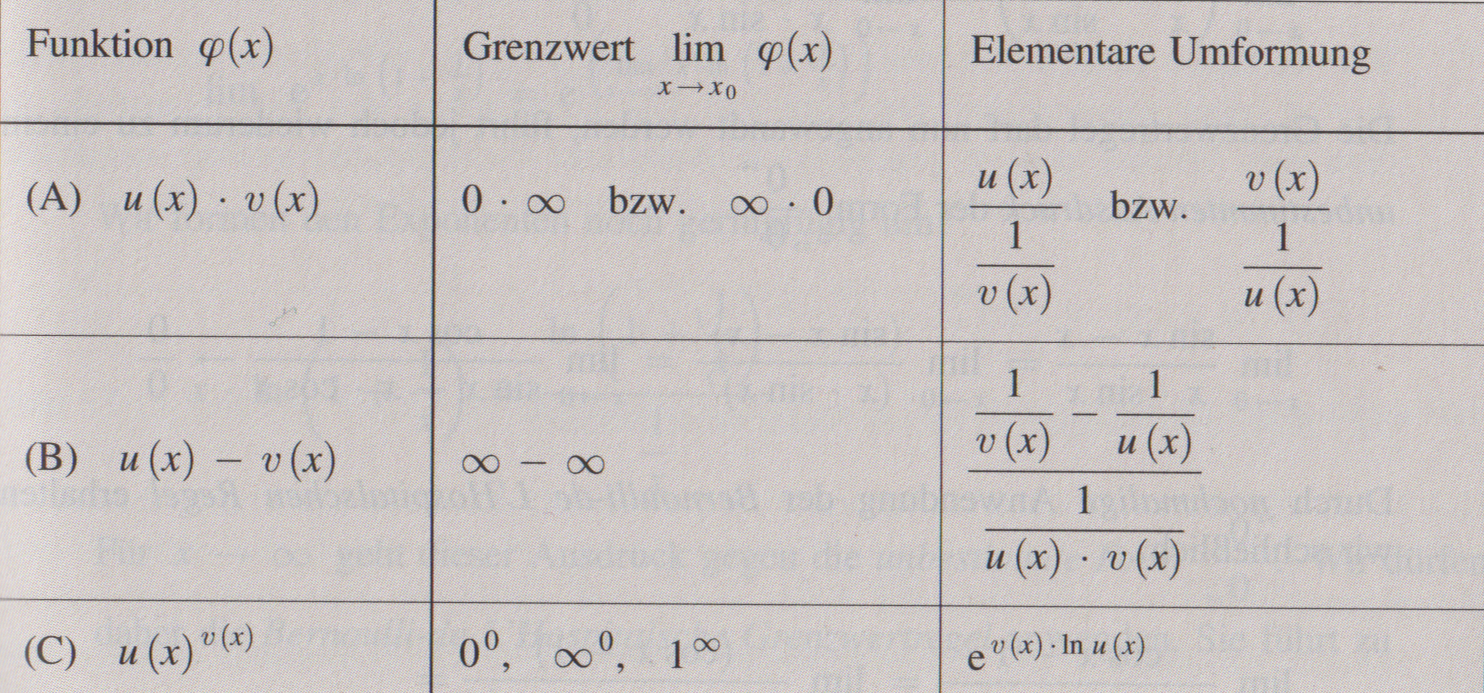
\includegraphics[width=1\textwidth]{Bilder/bdh-umformungstabelle}
\caption{Elementare Umformungen für unbestimmte Ausdrücke}
\end{figure} 
%\renewcommand{\arraystretch}{3}
